\documentclass[11pt]{report}
\usepackage[a4paper, total={6.0in, 9.0in}]{geometry}
\usepackage{amsmath,amsfonts,amsthm,amssymb}
\usepackage{fancyhdr}
\usepackage{color}
\usepackage{graphicx}
\usepackage{subcaption}
\usepackage{enumerate}
\usepackage{setspace}
\usepackage{listings,xcolor}
\usepackage{courier}
\usepackage{algorithm}
\usepackage{algorithmic}

\lstset{
  basicstyle=\small\linespread{1.4}\ttfamily,
  frame=tb,framextopmargin=5pt,framexbottommargin=5pt,
  numbers=left,numberstyle=\small\color{gray},
  showspaces=false,showtabs=false,showstringspaces=false,
  tabsize=4,rulecolor=\color{gray},
  xleftmargin=1.5em,numbersep=1.5em,
  breaklines=true,breakatwhitespace=true
}

\addtolength{\skip\footins}{1pc}  % add some space before main text and footnotes.

% Variables
\def\myTitleLineSpacing{2.5}
\def\myTocLineSpacing{1.5}
\def\myChapterLineSpacing{1.2}
\def\mySectionLineSpacing{1.2}
\def\myContentLineSpacing{1.8}

% Macros
\newcommand{\myChapter}[1]{

  \setstretch{\myChapterLineSpacing}\chapter{#1}
  \setstretch{\myContentLineSpacing}
}

\newcommand{\mySection}[1]{

  \setstretch{\mySectionLineSpacing}\section{#1}
  \setstretch{\myContentLineSpacing}
}


\begin{document}
\pagenumbering{gobble}  % disables page numbering

% Cover page
\setstretch{\myTitleLineSpacing}
\def\title{A Study on Roll Call Automation using Machine Learning and Face Recognition}
\def\author{Guan-Zhong Wang}
\def\supervisor{Prof. Chun-Ming Tsai}
\def\date{Feb 2020}

\begin{titlepage}
  \begin{center}
    \vspace*{3.5cm}

    \noindent\rule{16cm}{1.5pt}

    \vspace*{0.5cm}
    \textbf{\huge \title}
    \vspace*{0.5cm}
    \noindent\rule{16cm}{1.5pt}

    \vspace{0.5cm}
    {\large Presented by} \textbf{\Large \author}\\
    \vspace{0.3cm}
    {\large Supervised by} \textbf{\Large \supervisor}\\
    \vspace{1.2cm}

    \vspace{1.7cm}
    \includegraphics[width=0.3\textwidth]{figures/utaipei.png}
    \vspace{1.7cm}

    \vfill

    {\Large A thesis submitted to University of Taipei\\
      in partial fulfillment of the requirements for the degree of\\
      Bachelor of Science with a major in Computer Science\\
    }
    \vspace{1.2cm}
    {\Large \textbf\date}

    \vspace{3.5cm}

  \end{center}
\end{titlepage}

\newpage

% Table of Contents
\setstretch{\myTocLineSpacing}
\tableofcontents
\newpage

% Contents
\pagenumbering{arabic}  % enables page numbering
\setstretch{\myContentLineSpacing}
\begin{center}
  \section*{\abstractname}
\end{center}
\large

With the rapid advancements in technologies over the past few decades, facial recognition has become
ubiquitous in modern days. Despite being a relatively new technology, facial recognition has been
extensively employed in many products we use day-to-day. Large corporations, such as Google, Apple, Microsoft, 
have implemented biometric authentication in their products, enabling their users to incorporate
such features into their daily lives. Intelligence agencies as well as police agencies have been using
such technology to track down criminals and certain targets. Some governments have been using it to automate
border control and even on some trivial tasks such as identifying the text on car plates, reducing a huge amount
of tedious works that would have otherwise been carried out by human manually. Educational organizations
could also benefit from facial recognition by utilizing it to automate roll calls, allowing professors and teachers
to have more time to focus on teaching and allowing students to have more time to spend on learning during classes.
Traditionally, a teacher needs to call each student's name one by one in order to check who is present at a class,
and an entire semester could totally take 90 minutes if every semester consists of 18 weeks and each roll call takes
5 minutes to perform. In this thesis, we combined facial recognition as well as deep metric learning and proposed
a functional roll call automation system which can be practically employed in educational organizations, 
aiding professors to record student attendance. We will also evaluate the practicality of our method by comparing
similar approaches with our methods such as signing into classes by scanning students' ID cards, and
signing in to classes via mobile devices using GPS location tracking. The result of this research is expected to
reduce the chance of fraudulent class sign-ins that could arise in other similar methods, while ensuring the roll calls
could be smoothly automated by our system.
\newpage

\section{Introduction}
With the rapid growth of technology, more and more repetitive tasks can be automated by programs.
In my semester project, I built a system to replace the tedious procedure of a traditional roll call.
\newline

Initially, the users (typically teachers) are required to populate the database with the information
of the courses and students he/her teaches. Secondly, the users have to take several photos of each
student presented in the database and compute their facial embeddings. Lastly, the program can start
identifying students' faces and help users automate roll calls.
\newline

\section{Related Works}
Text

\subsection{Alternative Facial Recognition Approaches}
Text

\section{RFID Roll Call System}
Text

\subsection{Fingerprint Roll Call System}
Text


\myChapter{Proposed Roll Call System using Facial Recognition Technology}
In this chapter, we firstly discuss the usage of our roll call system, PyRollCall.
Next, we review the system analysis and design of our proposed roll call system,
and then go into the details of our system's implementation.

\mySection{System Overview}
Our system's primary goal is to help school faculties perform roll calls with ease.
Traditional roll calls require teachers to call the names of students individually to record students' attendance,
while PyRollCall let a teacher simply take a photo of the entire class and record students' attendance
using Facial Recognition, thus saving more time for both teachers and students in classes.
\vspace{0.5cm}

Before we can actually use the system to recognize the faces of students, teachers should
collect at least 10 to 15 photos for each student, and let the system compute the measurement (or embedding) of each face.
These pre-computed facial embeddings will be saved in the database for later use.
When a face is caputured in roll calls, the system will use k-NN classification and votes
to determine whom the face belongs to.
\vspace{0.5cm}

The user (usually a teacher) should enter the names of the courses into the system, as well as all students' names and IDs,
and for each course select which students are taking it. After entering these data into the system,
PyRollCall will be ready to perform roll call for a specific course using facial recognition.
To summarize, users should (1) collect approximately 10 to 15 photos for each student and
let PyRollCall pre-compute their facial embeddings, and (2) set up the courses' and students' data.
Figure~\ref{fig:systemAppearance} demonstrates the GUI used to manage the data of courses and students.
\vspace{0.8cm}

\begin{figure}[!htb]
  \centering
  \begin{subfigure}[b]{0.49\linewidth}
    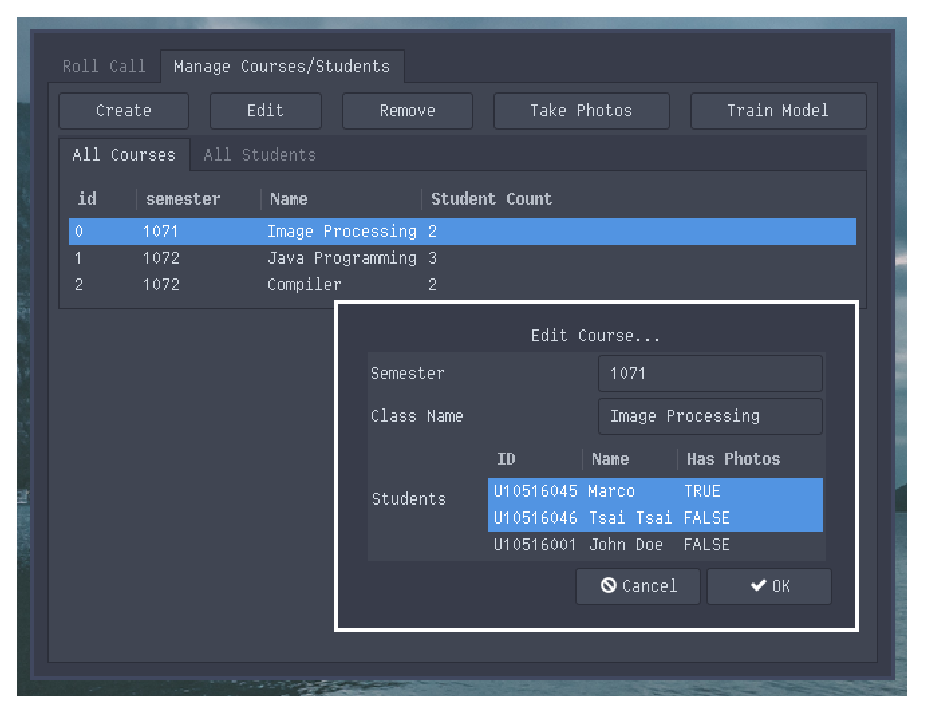
\includegraphics[width=\linewidth]{figures/preview1.eps}
    \caption{Managing courses.}
  \end{subfigure}
  \begin{subfigure}[b]{0.49\linewidth}
    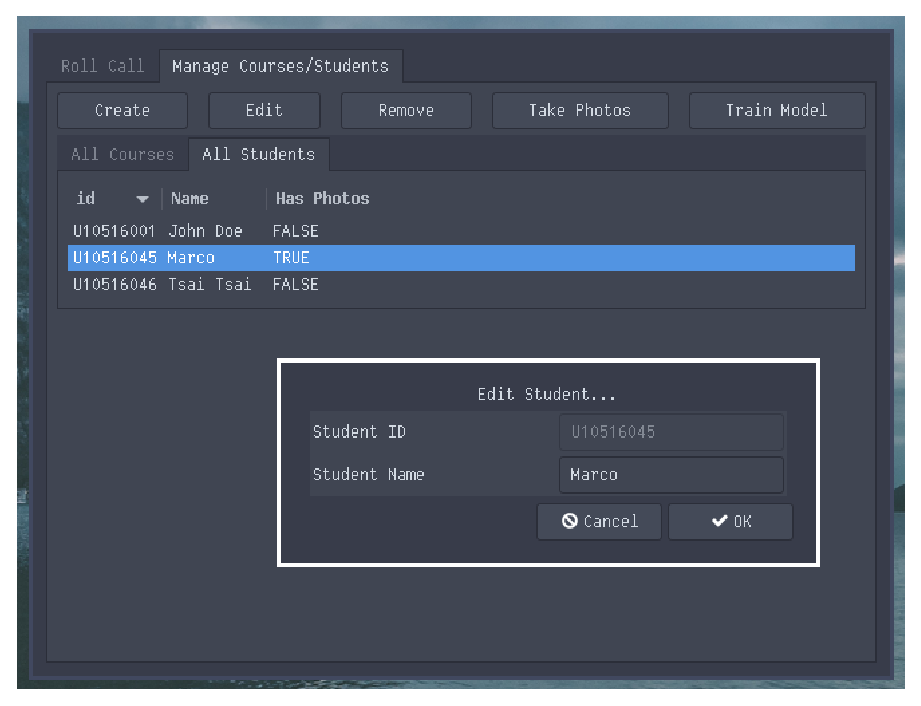
\includegraphics[width=\linewidth]{figures/preview2.eps}
    \caption{Managing students.}
  \end{subfigure}
  \caption{PyRollCall running on a Linux machine with X11\protect\footnotemark \ installed.}
  \label{fig:systemAppearance}
\end{figure}
\vspace{0.5cm}

\footnotetext{X11, also known as X Window System, or simply X, is a windowing system that provides the basic framework for building GUI environments.}

%Another usage of this system is taking the photo of each student one by one as long as
%the size of the class is small enough. If the size of the class is too large, this apparently
%can result in longer waiting time for the students, and hence this approach is impractical.
%Consequently, our main objective is to ensure that the system can accurately recognize all the faces
%in a large image as possible as it can.
%The actions available via PyRollCall's GUI are listed as follows:
%\vspace{0.5cm}

%\setstretch{0.8}
%\begin{itemize}
%  \item Maintain the data of the course and students they teach.
%  \item Take photos of students with a camera and compute the facial embeddings.
%  \item Perform roll calls for a specific course.
%  \item Export the results of roll calls to files.
%\end{itemize}
%\setstretch{\myContentLineSpacing}


%\vspace{0.5cm}
When a roll call ends, the system automatically exports a statistical report to a file.
These reports will be categorized nicely into different directories by date,
with the filename being the course name. Listing~\ref{lst:example-log} demonstrates
an example file containing the result of a roll call.
\clearpage

\begin{lstlisting}[numbers=none,xleftmargin=0em,caption={Layout of PyRollCall's root directory.},label={lst:example-log}]
$ cat logs/2019/01/01/Java.txt
Course Name: Java
Export Time: 2019/01/0120:37
Arrived: 8 / Late: 2 / 
Total: 10
Late Students: Tsai,John
\end{lstlisting}

Now that we have understood the prerequisites of the facial recognition features in PyRollCall,
it is time that we get to the installation details of this system. PyRollCall is able to run on Windows,
macOS and unix-like systems as long as the system supports Python 3 and GUI applications.
Furthermore, PyRollCall is open-source and managed with \emph{git}\footnote{git is a distributed
  version control system used for tracking file content changes in source code during software development},
and all of its external dependencies are already packaged in the project via Python's {virtualenv}\footnote{\
  virtualenv is a tool to create isolated Python environments by maintaining a set of libraries that a specific application depends on.},
thus the users do not have to worry about what and which versions of libraries they need to install. To checkout and run the project:

%Windows and macOS should natively support GUI applications. However, if you are running Linux,
%some distributions such as CentOS, Arch and Gentoo might not, by default, support
%GUI applications. In this case, you'll have to manually install X11 packages on your system.


\begin{lstlisting}[numbers=none,xleftmargin=0em,caption={Shell commands to checkout and run PyRollCall}]
$ git clone https://github.com/aesophor/pyrollcall.git
$ cd pyrollcall
$ source venv/bin/activate
$ ./pyrollcall.py 
\end{lstlisting}

The entry point to the system is \emph{pyrollcall.py}, a script located under the project's root directory.
Before running it, source the shell script \emph{venv/bin/activate} to activate the project's virtual environment.
\clearpage

\mySection{System Analysis and Design}
Text

\begin{figure}[!htb]
  \centering
  \includegraphics[width=\linewidth]{figures/use-case.png}
  \caption{Use Case Diagram}
  \label{fig:implementation}
\end{figure}

\begin{figure}[!htb]
  \centering
  \includegraphics[width=\linewidth]{figures/system-architecture.png}
  \caption{System Architecture}
  \label{fig:implementation}
\end{figure}

\mySection{Implementation}
Text

\begin{algorithm}
\caption{A}
\label{alg:A}
\begin{algorithmic}
\STATE {set $r(t)=x(t)$}
\REPEAT
\STATE set $h(t)=r(t)$
\REPEAT
\STATE set $h(t)=r(t)$
\UNTIL{B}
\UNTIL{B}
\end{algorithmic}
\end{algorithm}

\begin{figure}[!htb]
  \centering
  \includegraphics[width=\linewidth]{figures/system-architecture.png}
  \caption{System Architecture}
  \label{fig:implementation}
\end{figure}


\myChapter{Experiments and Results}
In this chapter, we assess the accuracy and practicality of PyRollCall. We briefly explain
the image sets and parameters used in our experiments, then we present and discuss
the experimental results.

\mySection{Experimental Settings}
In this section, we assess the practicality of PyRollCall. Two of the most important
functionalities of a facial recognition roll call system are: (1) face detection
and (2) facial recognition. If these two features work accurately, then the system
is considered to be working as intended. Firstly, we evaluate the performance of face detection.
Figure~\ref{fig:face-detection-test} shows that PyRollCall is able to detect all faces
within the image regardless of head tilt, rotation and even facial expressions.
\vspace{0.2cm}

\begin{figure}[!htb]
  \centering
  \includegraphics[height=8.5cm]{figures/face-detection-test.png}
  \caption{Face Detection}
  \label{fig:face-detection-test}
\end{figure}

In our experiments, all faces are facing upfront to the camera, and thus the successful
rate of face detection is rather high. In real-world scenarios, the faces of students
may be turned into various angles and the results of face detection will vary. Hence,
when taking photos from the students, the teacher will have to ask for the attention from
the students for a few seconds.

\mySection{Experimental Results}
With sufficient photos of students provided and their facial embeddings pre-computed,
the system will be able to detect and recognize faces correctly. However, to save time
in classes, teachers and students will have to spend equivilently extra amount of time
before classes on the tasks such as collecting photos and pre-computing facial embeddings.
This proves that there is a trade off between convenience and efficiency.


\myChapter{Conclusion and Future Research}

\mySection{Conclusion}
In this thesis, we have proposed a roll call system using Deep Metric Learning and k-NN classification.
The system enables educational organizations to record students' attendance simply by taking a photo of
the entire classroom, thus saving a huge amount of time for both teachers and students.
We have also evaluated the practicality of our system by examining the accuracy of facial recognition.
\vspace{0.5cm}

Implemented in Python 3.5 and with the help of \emph{virtualenv}, PyRollCall is cross-platform and highly portable,
since all of its dependencies are already packaged with the project. It is implemented with \emph{OpenCV}
for capturing images from a camera, with \emph{face\_recognition} which is a wrapper library of \emph{dlib}
for performing facial recognition with Deep Metric Learning, and with \emph{PyGTK} for designing a user-friendly GUI.
\vspace{0.5cm}

There are two prerequisites which should be fulfilled before using PyRollCall:

\begin{enumerate}
  \item The user should enter the data of all students and courses he or she teaches into the system; for each course, select the students that are currently taking it.
  \item Collect approximately 10 to 15 photos from each student and let the system pre-compute their facial embeddings (or encodings).
\end{enumerate}

\input{chapters/conclusion-and-future-research/future-research}

\begin{thebibliography}{10}
  \addcontentsline{toc}{chapter}{Bibliography}

  \bibitem{wem-2018}
  William E. Miller (2018).
  Utilizing Facial Recognition Software to Record Classroom Attendance.

  \bibitem{chc-2012}
  Ching Hisang Chang (2012).
  Smart Classroom Roll Caller System with IOT Architecture.

  \bibitem{zuvio-irs}
  Zuvio IRS,
  An Interactive Educational Tool for Universities.
  \\\texttt{https://www.zuvio.com.tw/student}

  \bibitem{opencv}
  OpenCV (Open Source Computer Vision Library),
  A cross-platform Computer Vision and Machine Learning Library.
  \\\texttt{https://opencv.org/}

  \bibitem{dlib}
  Davis King.
  Dlib,
  A C++ Toolkit Containing Machine Learning Algorithms and Tools to Solve Complex Real World Problems.
  \\\texttt{http://dlib.net/}

  \bibitem{face-recognition}
  Adam Geitgey.\
  face\_recognition,
  The World's Simplest Facial Recognition API for Python and the Command Line.
  \\\texttt{https://github.com/ageitgey/face\_recognition}

  \bibitem{pygtk}
  PyGTK,
  A Convenient Wrapper for GTK+ Library for Use in Python Programs.
  \\\texttt{https://wiki.gnome.org/Projects/PyGTK}

  \bibitem{adrian}
  Adrian Rosebrock (2018).
  Face Recognition with OpenCV, Python, and Deep Learning.
  \\\texttt{https://www.pyimagesearch.com/2018/06/18/face-recognition\-with-opencv-python-and-deep-learning/}

  \bibitem{bib1}
  Himanshu Mallik (2015).
  An Automated Student Attendance Registering System using Face Recognition.

  \bibitem{bib2}
  Abidi, M.A. and Gonzalez, R. C. (1992).
  Data Fusion in Robotics and Machine Intelligence.
  Academic Press, New York.

  \bibitem{bib3}
  Abramson, N. (1963).
  Information Theory and Coding.
  McGraw-Hill, New York.

  \bibitem{bib4}
  Md. Shafiqul Islam, Asif Mahmud, Azmina Akter Papeya, Irin Sultana Onny (2017).
  Real Time Classroom Attendance Management System.

  \bibitem{err-facial-recog-tech}
  AFP (2019)
  Bangkok Post
  \\\texttt{https://www.bangkokpost.com/tech/1820554/study-finds-massive-errors-in-facial-recognition-tech}

\end{thebibliography}


\end{document}
